% Provenance (never printed): old premiere S material on the lithosphere and the
% asthenosphere (chemical and mechanical layers, the low-velocity zone, the
% geotherm, isostasy); see sources/book2/PROVENANCE.md. S speeds from
% figdata/grade-11/prem_profiles.py (part upper), the geotherm and the solidus
% from geotherm_solidus.py, the elevations from hypsometry.py (ETOPO1).
% Glacial rebound belongs to g12; lithostatic pressure (term) to g12.
\chapter{Lithosfeer en asthenosfeer}\label{ch:g11:lithosphere-asthenosphere}

Negen tiende van een ijsberg ligt onder water: het ijs drijft omdat het iets
minder dicht is dan de zee, en het zakt in het water tot het water dat het
wegduwt evenveel weegt als de hele ijsberg. Bergketens gedragen zich op
ongeveer dezelfde manier. Onder de hoogste ervan is de korst bijna twee keer zo
dik als gewoonlijk, en het grootste deel van die extra korst zit verborgen
eronder, zoals het ijs onder de waterlijn. Maar een ijsberg drijft in een
vloeistof, en de mantel onder een bergketen is vast gesteente. Dit hoofdstuk laat
zien hoe een vaste stof zich kan gedragen als een vloeistof waarop de buitenste
schil van de Aarde drijft, en wat die schil is.
% ledger: usgs:ice-density, karplus:tibet-moho, cm95:crust

\begin{recall}
De Aarde heeft een aardkorst, een mantel en een kern (Boek 1, jaar 6). De \omterm{def:g11:seismic-structure:moho}{Moho},
aan de onderkant van de korst, ligt onder de continenten gemiddeld ongeveer
\qty{41}{km} diep en een paar kilometer onder de oceaanbodem; seismische snelheden
en dichtheden zijn op elke diepte bekend uit een \omterm{def:g11:seismic-structure:reference-model}{referentiemodel van de Aarde}
(\cref{ch:g11:seismic-structure}). Het gesteente wordt warmer met de diepte, met
ongeveer 25 tot \qty{30}{\celsius} per kilometer dicht bij het oppervlak (Boek 1,
jaar 6). Een voorwerp dat in een vloeistof drijft, verplaatst een gewicht aan
vloeistof dat gelijk is aan zijn eigen gewicht, en de druk aan de onderkant van een
kolom materiaal is het gewicht van de kolom gedeeld door haar oppervlakte (de
natuurkundeboeken).
\end{recall}
% ledger: cm95:crust, usgs:crust-thickness, usgs:gradient-29 (Book 1 rows)

\begin{omfigure}
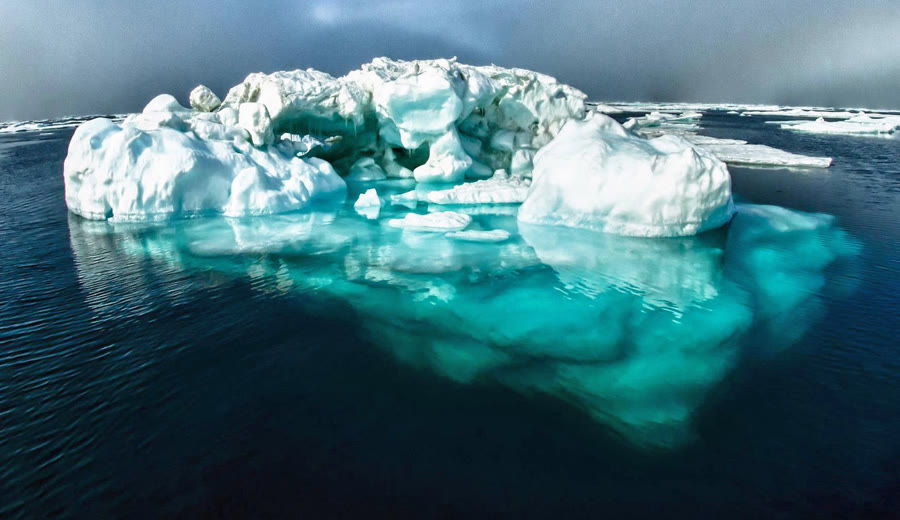
\includegraphics[width=0.66\linewidth]{images/book2/g11-noaa-iceberg.jpg}

{\small Een ijsberg gezien van net boven het water: het ijs onder het oppervlak,
dat door de heldere zee heen schijnt, is veel groter dan het deel in de lucht.
Foto: NOAA (publiek domein).}
\end{omfigure}
% ledger: photo:g11-iceberg

\section{Twee manieren om de Aarde in lagen te verdelen}

De korst, de mantel en de kern zijn lagen van verschillende
\emph{materialen}: de korst bestaat uit gesteenten die rijk zijn aan silicium,
aluminium en zuurstof, de mantel uit een dichter gesteente, de kern uit metaal.
Maar het buitenste deel van de Aarde kan ook worden ingedeeld naar hoe het
gesteente zich \emph{gedraagt} wanneer er heel lang krachten op werken.

\begin{definition}[Lithosfeer; asthenosfeer]\label{def:g11:lithosphere-asthenosphere:lithosphere}
De \emph{lithosfeer}\index{lithosfeer} is de starre buitenste schil van de Aarde:
de korst en het bovenste, koudste deel van de mantel, die samen in de tektonische
platen breken en niet vloeien. De
\emph{asthenosfeer}\index{asthenosfeer} is de laag van de mantel onder de
lithosfeer, heter en zwakker, die over lange tijdspannen langzaam vloeit, als een
heel stijve pasta.
\end{definition}

De grens tussen de twee ligt onder de oceanen en de meeste continenten ongeveer
70 tot \qty{100}{km} diep, en dieper onder de oudste delen van de continenten;
in de Verenigde Staten is de \omterm{def:g11:lithosphere-asthenosphere:lithosphere}{lithosfeer} bijvoorbeeld van ongeveer \qty{40}{km}
dik in het westen tot meer dan \qty{200}{km} dik in het midden van het continent.
De onderkant van de \omterm{def:g11:lithosphere-asthenosphere:lithosphere}{lithosfeer} is niet de \omterm{def:g11:seismic-structure:moho}{Moho}: het grootste deel van de
\omterm{def:g11:lithosphere-asthenosphere:lithosphere}{lithosfeer} is mantelgesteente.
% ledger: rs09:lab, fischer:lab, porter:lab, usgs:lithosphere-80km (Book 1 row)

\begin{omfigure}
\begin{tikzpicture}[x=1cm, y=-0.0125cm, font=\footnotesize]
% depths to scale: crust 41 km (cm95:crust), lithosphere 100 km (rs09:lab), 0-400 km
  \shade[top color=omLithPeridotite!70, bottom color=omLithPeridotite!25] (5,100) rectangle (8,400);
  \fill[omLithGranite!55] (0,0) rectangle (3,41);
  \fill[omLithPeridotite!55] (0,41) rectangle (3,400);
  \fill[black!25] (5,0) rectangle (8,100);
  \draw (0,0) rectangle (3,400);
  \draw (5,0) -- (5,400) (8,0) -- (8,400) (5,0) -- (8,0);
  \draw[line width=0.8pt] (0,41) -- (3,41);
  \draw[line width=0.8pt, densely dashed] (5,100) -- (8,100);
  \draw[densely dotted, black!60] (3,41) -- (5,41);
  \node at (1.5,20) {korst};
  \node[align=center] at (1.5,220) {mantel};
  \node[align=center] at (6.5,50) {lithosfeer\\star};
  \node[align=center] at (6.5,180) {asthenosfeer\\zwak, vloeit langzaam};
  \node[align=center, text=black!70] at (6.5,340) {diepere mantel};
  \node[anchor=south, font=\small] at (1.5,0) {naar materiaal};
  \node[anchor=south, font=\small] at (6.5,0) {naar gedrag};
  \foreach \d in {0,100,200,300,400} {\draw (-0.1,\d) -- (0,\d); \node[anchor=east] at (-0.1,\d) {\d};}
  \node[anchor=east, rotate=90, anchor=south] at (-0.9,200) {diepte (\unit{km})};
  \node[anchor=south, font=\scriptsize, align=center] at (4,41) {Moho\\(\qty{41}{km})};
  \node[anchor=west, align=left] at (8.15,100) {onderkant van de\\lithosfeer\\(ongeveer \qty{100}{km})};
\end{tikzpicture}

{\small De bovenste \qty{400}{km} van de Aarde onder een continent, op schaal.
Links: de lagen naar materiaal. Rechts: de lagen naar gedrag. De starre
\omterm{def:g11:lithosphere-asthenosphere:lithosphere}{lithosfeer} omvat de hele korst en de bovenkant van de mantel; de \omterm{def:g11:lithosphere-asthenosphere:lithosphere}{asthenosfeer}
heeft geen scherpe ondergrens.}
\end{omfigure}

\section{De lagesnelheidszone}

Seismische golven laten de \omterm{def:g11:lithosphere-asthenosphere:lithosphere}{asthenosfeer} zien. Bijna overal in de Aarde nemen
seismische snelheden toe met de diepte, omdat het gesteente steeds meer wordt
samengedrukt. Onder de \omterm{def:g11:lithosphere-asthenosphere:lithosphere}{lithosfeer} gebeurt het omgekeerde.

\begin{definition}[Lagesnelheidszone]\label{def:g11:lithosphere-asthenosphere:lvz}
De \emph{lagesnelheidszone}\index{lagesnelheidszone} is de laag van de bovenmantel,
onder de \omterm{def:g11:lithosphere-asthenosphere:lithosphere}{lithosfeer}, waarin seismische golven trager gaan dan in het gesteente
erboven en eronder.
\end{definition}

In het \omterm{def:g11:seismic-structure:reference-model}{referentiemodel van de Aarde} daalt de S-snelheid langzaam van de \omterm{def:g11:seismic-structure:moho}{Moho} tot
\qty{220}{km}, en springt dan omhoog. Seismische studies over de hele wereld vinden
ergens tussen 70 en \qty{100}{km} een scherpe daling van de snelheid: de bovenkant
van de \omterm{def:g11:lithosphere-asthenosphere:lithosphere}{asthenosfeer}. Het gesteente is daar heet genoeg om dicht bij het smelten te
zijn, en kan een heel klein beetje smelt bevatten; het kan ook meer water bevatten
dan het gesteente erboven. Gesteente dat dicht bij het smelten is, is zwak: het
vertraagt seismische golven, en het kan vloeien.
% ledger: data:prem, rs09:lab, fischer:lab, porter:lab

\begin{omfigure}
\begin{tikzpicture}
\begin{axis}[omrecord, omdepth, width=0.6\linewidth, height=6.0cm, xmin=3.0, xmax=5.0, ymin=0, ymax=400,
  xlabel={S-snelheid (\unit{km/s})}, ylabel={diepte (\unit{km})}, xtick={3.0,3.5,...,5.0},
  xticklabel style={/pgf/number format/fixed, /pgf/number format/precision=1},
  tick label style={font=\small}, label style={font=\small}]
% computed in figdata/grade-11/prem_profiles.py (part upper); ledger: data:prem
\fill[black!10] (axis cs:3.0,80) rectangle (axis cs:5.0,220);
\addplot[omProp, line width=0.9pt] table[x=vs, y=depth] {figdata/out/grade-11-prem_profiles-upper.dat};
\node[font=\scriptsize, anchor=west, align=left] at (axis cs:3.1,150) {lagesnelheids-\\zone};
\node[font=\scriptsize, anchor=west] at (axis cs:3.95,12) {korst};
\end{axis}
\end{tikzpicture}

{\small De S-snelheid in de bovenste \qty{400}{km} van het \omterm{def:g11:seismic-structure:reference-model}{referentiemodel van de
Aarde}. Onder de korst neemt de snelheid langzaam af met de diepte tot
\qty{220}{km} (gearceerd vanaf \qty{80}{km}), en neemt ze daarna met plotselinge
sprongen weer toe.}
\end{omfigure}

\section{De geotherm}

\begin{definition}[Geotherm; geothermische gradiënt]\label{def:g11:lithosphere-asthenosphere:geotherm}
Een \emph{geotherm}\index{geotherm} is de kromme van de temperatuur tegen de diepte
onder een plaats. De \emph{geothermische gradiënt}\index{geothermische gradient@geothermische gradiënt}
is de stijging van de temperatuur per eenheid van diepte, in graden per kilometer.
\end{definition}

Boorgaten meten de \omterm{def:g11:lithosphere-asthenosphere:geotherm}{geotherm} alleen in de eerste paar kilometer, waar de
temperatuur met 25 tot \qty{30}{\celsius} per kilometer stijgt (Boek 1,
jaar 6). Dieper wordt hij berekend uit de warmte die door het oppervlak naar
buiten stroomt en uit de eigenschappen van de gesteenten;
\cref{ch:g12:internal-heat} laat zien waar die warmte vandaan komt. Twee feiten
bepalen het resultaat. Een deel van de warmte wordt in de bovenkorst zelf
gemaakt, dus de gradiënt is het steilst dicht bij het oppervlak en kleiner onder
de korst. En in de \omterm{def:g11:lithosphere-asthenosphere:lithosphere}{asthenosfeer}, die vloeit, voert de langzame beweging van het
gesteente de warmte mee en egaliseert ze de temperatuur: die stijgt er maar
ongeveer \qty{0.45}{\celsius} per kilometer. De onderkant van de \omterm{def:g11:lithosphere-asthenosphere:lithosphere}{lithosfeer} wordt
gelegd waar de steile \omterm{def:g11:lithosphere-asthenosphere:geotherm}{geotherm} van de \omterm{def:g11:lithosphere-asthenosphere:lithosphere}{lithosfeer} de vlakke van de \omterm{def:g11:lithosphere-asthenosphere:lithosphere}{asthenosfeer}
ontmoet, bij ongeveer \qty{1300}{\celsius}.
% ledger: usgs:gradient-29 (Book 1 row), b2dd10:continents, b2roy:provinces, roy:conductivity,
% katsura10:adiabat, porter:lab

\begin{omfigure}
\begin{tikzpicture}
\begin{axis}[omrecord, omdepth, width=0.7\linewidth, height=6.4cm, xmin=0, xmax=2000, ymin=0, ymax=300,
  xlabel={temperatuur (\unit{\celsius})}, ylabel={diepte (\unit{km})}, xtick={0,500,...,2000},
  tick label style={font=\small}, label style={font=\small}]
% computed in figdata/grade-11/geotherm_solidus.py; ledger: b2dd10:continents, b2roy:provinces,
% roy:conductivity, porter:lab, katsura10:adiabat, hirschmann:solidus, data:prem
\fill[black!8] (axis cs:0,99.7) rectangle (axis cs:2000,300);
\addplot[omDef, line width=1.0pt] table[x=t_geotherm, y=depth_km] {figdata/out/grade-11-geotherm_solidus-geotherm.dat};
\addplot[omDef, densely dashed, restrict y to domain=99:300] table[x=t_cond, y=depth_km] {figdata/out/grade-11-geotherm_solidus-geotherm.dat};
\addplot[omProp, line width=1.0pt] table[x=t_solidus, y=depth_km] {figdata/out/grade-11-geotherm_solidus-geotherm.dat};
\draw[black!60] (axis cs:0,99.7) -- (axis cs:2000,99.7);
\node[font=\scriptsize, anchor=south west] at (axis cs:20,99.7) {onderkant van de lithosfeer};
\node[font=\scriptsize, anchor=north west] at (axis cs:20,102) {asthenosfeer};
\node[font=\scriptsize, text=omDef, anchor=north west] at (axis cs:480,6) {geotherm};
\node[font=\scriptsize, text=omProp, anchor=west] at (axis cs:1300,22) {begin van smelten};
\end{axis}
\end{tikzpicture}

{\small Een modelgeotherm onder een continent (blauw) en de temperatuur waarbij
mantelgesteente (peridotiet, zonder water) begint te smelten (oranje). De
\omterm{def:g11:lithosphere-asthenosphere:geotherm}{geotherm} is berekend uit de gemiddelde warmtestroom van de continenten en gemeten
eigenschappen van gesteenten; in de \omterm{def:g11:lithosphere-asthenosphere:lithosphere}{asthenosfeer} (grijs) stijgt hij langzaam. De
stippellijn toont hoe de steilere stijging van de \omterm{def:g11:lithosphere-asthenosphere:lithosphere}{lithosfeer} zou doorlopen. De
twee krommen komen het dichtst bij elkaar, ongeveer \qty{140}{\celsius} uit
elkaar, bij de onderkant van de \omterm{def:g11:lithosphere-asthenosphere:lithosphere}{lithosfeer}.}
\end{omfigure}
% values: lab_km 99.7, t_lab_c 1345, closest_gap_c 144 (figdata/grade-11/geotherm_solidus.py)

De smelttemperatuur van het mantelgesteente stijgt met de diepte, omdat het
gesteente steeds meer wordt samengedrukt (Boek 1, jaar 6): ongeveer
\qty{1120}{\celsius} aan het oppervlak, bijna \qty{1500}{\celsius} op
\qty{100}{km}. In het model komt de \omterm{def:g11:lithosphere-asthenosphere:geotherm}{geotherm} er net onder de \omterm{def:g11:lithosphere-asthenosphere:lithosphere}{lithosfeer} het
dichtst bij, ongeveer \qty{140}{\celsius} eronder. Een beetje water, of een iets
hetere mantel, overbrugt dat verschil: in het westen van de Verenigde Staten, waar
de \omterm{def:g11:lithosphere-asthenosphere:lithosphere}{lithosfeer} dun is, is een klein deel van de mantel eronder gedeeltelijk gesmolten.
% ledger: hirschmann:solidus, porter:lab; computed in figdata/grade-11/geotherm_solidus.py
% (solidus0_c 1120.7, solidus100_c 1489, closest_gap_c 144)

\section{Isostasie}

\subsection{Drijven op een vaste stof}

Over de paar seconden van een aardbevingsgolf is de \omterm{def:g11:lithosphere-asthenosphere:lithosphere}{asthenosfeer} een vaste stof.
Over lange tijdspannen vloeit ze. Een last die op de \omterm{def:g11:lithosphere-asthenosphere:lithosphere}{lithosfeer} wordt gelegd ---
een bergketen, een ijskap --- duwt de \omterm{def:g11:lithosphere-asthenosphere:lithosphere}{asthenosfeer} langzaam opzij tot de last
drijft, zoals een blok hout op water.

\begin{definition}[Isostasie; compensatiediepte]\label{def:g11:lithosphere-asthenosphere:isostasy}
\emph{Isostasie}\index{isostasie} is het evenwicht waarin de buitenste lagen van de
Aarde op de \omterm{def:g11:lithosphere-asthenosphere:lithosphere}{asthenosfeer} drijven: op een diepte in de mantel die de
\emph{compensatiediepte}\index{compensatiediepte} heet, heeft elke kolom gesteente
met dezelfde doorsnede, van het oppervlak tot die diepte, hetzelfde gewicht,
welk reliëf er ook boven ligt.
\end{definition}

\begin{omfigure}
\begin{tikzpicture}[x=1cm, y=1cm, font=\footnotesize, >={Stealth[length=4pt]}]
% not to scale
  \fill[omSea!50] (6,0) rectangle (8.6,-0.9);
  \fill[omLithPeridotite!45] (0,-5.2) rectangle (2.6,-6.6);
  \fill[omLithGranite!55] (0,2.0) -- (2.6,2.0) -- (2.6,-5.2) -- (0,-5.2) -- cycle;
  \fill[omLithGranite!55] (2.6,0) rectangle (6,-3.0);
  \fill[omLithGranite!55] (6,-0.9) rectangle (8.6,-1.6); % same fill: one crustal density in Airy's model
  \fill[omLithPeridotite!45] (2.6,-3.0) rectangle (6,-6.6);
  \fill[omLithPeridotite!45] (6,-1.6) rectangle (8.6,-6.6);
  \draw (0,2.0) -- (2.6,2.0) -- (2.6,0) -- (6,0);
  \draw (6,0) -- (8.6,0);
  \draw[line width=0.8pt] (0,-5.2) -- (2.6,-5.2) -- (2.6,-3.0) -- (6,-3.0) -- (6,-1.6) -- (8.6,-1.6);
  \draw[densely dashed, line width=0.8pt] (0,-6.2) -- (8.6,-6.2);
  \node[anchor=north east] at (8.6,-6.6) {compensatiediepte};
  \draw[black!50, densely dotted] (-0.2,0) -- (0,0);
  \node[anchor=east] at (-0.2,0) {zeeniveau};
  \node at (1.3,-1.6) {korst};
  \node at (4.3,-1.5) {korst};
  \node at (7.3,-0.45) {oceaan};
  \node at (7.3,-1.25) {korst};
  \node at (4.3,-4.8) {mantel};
  \node[anchor=south] at (1.3,2.0) {bergketen};
  \node[anchor=south] at (4.3,0) {laagland};
  \draw[<->] (2.75,0) -- (2.75,2.0); \node[anchor=west] at (2.8,1.0) {$h$};
  \draw[<->] (2.75,-3.0) -- (2.75,-5.2); \node[anchor=west] at (2.8,-4.1) {wortel $r$};
  \draw[<->] (5.85,0) -- (5.85,-3.0); \node[anchor=east] at (5.8,-1.0) {$T$};
\end{tikzpicture}

{\small Het model van Airy voor \omterm{def:g11:lithosphere-asthenosphere:isostasy}{isostasie} (niet op schaal). De korst heeft overal
dezelfde dichtheid; waar ze hoog staat, is ze dik en heeft ze een wortel die diep
in de dichtere mantel reikt. Onder de oceaan is de korst dun. Alle drie de
kolommen wegen tot de \omterm{def:g11:lithosphere-asthenosphere:isostasy}{compensatiediepte} evenveel.}
\end{omfigure}

\subsection{De wortel van een bergketen}

\begin{proposition}[Isostasie van Airy]\label{prop:g11:lithosphere-asthenosphere:airy}
Laat de korst een uniforme dichtheid $\rho_c$ hebben, en de mantel eronder een
dichtheid $\rho_m > \rho_c$. Als een gebied een hoogte $h$ boven een ander gebied
uitsteekt en beide in isostatisch evenwicht zijn, is zijn korst dikker met
\[
  \Delta H = h\,\frac{\rho_m}{\rho_m - \rho_c},
\]
waarvan $h$ boven het andere gebied uitsteekt en een wortel
$r = h\,\rho_c/(\rho_m - \rho_c)$ onder zijn korst reikt.\index{isostasie van Airy}
\end{proposition}

\begin{proof}
Neem twee kolommen met dezelfde oppervlakte $S$: het laagland met een korst van
dikte $T$, en de keten, waarvan de korst $h$ hoger staat en $r$ dieper reikt,
zodat haar dikte $T + h + r$ is. Tot een \omterm{def:g11:lithosphere-asthenosphere:isostasy}{compensatiediepte} onder beide \omterm{def:g11:seismic-structure:moho}{Moho}'s
heeft de kolom van de keten $h + r$ meer korst; de kolom van het laagland heeft
in plaats daarvan mantel over de dikte $r$. Met $g$ de valversnelling zijn de twee
gewichten gelijk als
\[
  \rho_c\,(h + r)\,S\,g = \rho_m\,r\,S\,g,
  \qquad\text{dat wil zeggen}\qquad
  r = h\,\frac{\rho_c}{\rho_m - \rho_c}.
\]
De korst is dikker met $h + r = h\,\bigl(1 + \rho_c/(\rho_m - \rho_c)\bigr)
= h\,\rho_m/(\rho_m - \rho_c)$.
\end{proof}

Met de gemiddelde dichtheid van de continentale korst, $\rho_c =
\qty{2830}{kg/m^3}$, en die van de mantel net onder de \omterm{def:g11:seismic-structure:moho}{Moho}, $\rho_m =
\qty{3380}{kg/m^3}$, is de wortel $2830/550 \approx 5.1$ keer de hoogte,
en is de korst ongeveer $6.1$ keer de hoogte dikker: een keten die
\qty{3}{km} boven haar omgeving uitsteekt, heeft een wortel van ongeveer \qty{15}{km}.
% ledger: cm95:crust, data:prem (rho 3.38 below the Moho)

\begin{method}[Een wortel berekenen]\label{met:g11:lithosphere-asthenosphere:root}
\begin{enumerate}
  \item Zoek de hoogte $h$ van het gebied boven een referentiegebied waarvan de
        korstdikte bekend is.
  \item Bereken $\rho_m/(\rho_m - \rho_c)$ met de dichtheden van korst en
        mantel.
  \item De korst is dikker dan de referentiekorst met $h\,\rho_m/(\rho_m -
        \rho_c)$; de wortel alleen is dat min $h$.
\end{enumerate}
\end{method}

\begin{example}[Een plateau van \qty{2}{km} hoog]\label{ex:g11:lithosphere-asthenosphere:plateau}
Een plateau steekt \qty{2}{km} uit boven een laagland waarvan de korst \qty{37}{km}
dik is. Zijn korst is dikker met $2 \times 3380/550 \approx \qty{12.3}{km}$:
in totaal ongeveer \qty{49}{km}, met een wortel van ongeveer \qty{10}{km}.
\end{example}

\subsection{Waarom de continenten hoog liggen}

\begin{definition}[Hypsometrische kromme]\label{def:g11:lithosphere-asthenosphere:hypsometry}
De \emph{hypsometrische kromme}\index{hypsometrische kromme} van de Aarde geeft
voor elke hoogte het deel van het aardoppervlak dat hoger ligt. Haar helling laat
zien hoeveel van het oppervlak op elke hoogte ligt.
\end{definition}

Als het oppervlak door toeval was gevormd, zou het grootste deel ervan dicht bij
één gemiddeld niveau liggen. Dat is niet zo.

\begin{proposition}[Twee niveaus]\label{prop:g11:lithosphere-asthenosphere:two-levels}
De hoogten van het aardoppervlak groeperen zich rond twee niveaus: een binnen een
paar honderd meter van zeeniveau, op de continenten, en een ongeveer 4 tot
\qty{5}{km} onder zeeniveau, op de diepe oceaanbodem. Land bedekt \qty{29}{\percent}
van het oppervlak; meer dan de helft van het oppervlak ligt dieper dan \qty{3}{km}
onder zeeniveau, en maar \qty{3}{\percent} rijst hoger op dan \qty{2}{km}.
\end{proposition}
% computed in figdata/grade-11/hypsometry.py from ETOPO1 (land_fraction 0.290,
% share_below_3000_pct 53.4, share_above_2000_pct 3.1; modes at +250 and -4250 m); ledger: data:etopo1

\begin{omfigure}
\begin{tikzpicture}
\begin{axis}[omrecord, width=0.86\linewidth, height=5.4cm, xmin=-11000, xmax=9000, ymin=0, ymax=18,
  xlabel={hoogte (\unit{m}; negatief: onder zeeniveau)}, ylabel={deel van het oppervlak (\unit{\percent})},
  xtick={-10000,-8000,...,8000}, scaled x ticks=false, xticklabel style={/pgf/number format/1000 sep={\,}, font=\scriptsize},
  tick label style={font=\small}, label style={font=\small}, clip=false]
% computed in figdata/grade-11/hypsometry.py; ledger: data:etopo1
\addplot[ybar interval, fill=omSea!70, draw=black!50, restrict expr to domain={\thisrow{land}}{0:0}] table[x=lo, y=share_pct] {figdata/out/grade-11-hypsometry-bins.dat};
\addplot[ybar interval, fill=omHypsLandC, draw=black!50, restrict expr to domain={\thisrow{land}}{1:1}] table[x=lo, y=share_pct] {figdata/out/grade-11-hypsometry-bins.dat};
\draw[black!60, densely dotted] (axis cs:0,0) -- (axis cs:0,18);
\node[font=\scriptsize, anchor=south west] at (axis cs:600,15.5) {continenten};
\node[font=\scriptsize, anchor=south] at (axis cs:-4250,12.2) {diepe oceaanbodem};
\end{axis}
\end{tikzpicture}

{\small Deel van het aardoppervlak in elke band van \qty{500}{m} hoogte (uit
ETOPO1, per graad; boven Antarctica en Groenland de bovenkant van het ijs). De
twee pieken zijn de continenten en de diepe oceaanbodem.}
\end{omfigure}

\omterm{def:g11:lithosphere-asthenosphere:isostasy}{Isostasie} verklaart de twee niveaus. De continenten bestaan uit een dikke korst,
gemiddeld ongeveer \qty{41}{km}, van licht gesteente; de oceaanbodem uit een dunne
korst van dichter gesteente, maar ongeveer \qty{5}{km} dik. Beide drijven op de
\omterm{def:g11:lithosphere-asthenosphere:lithosphere}{asthenosfeer}: de dikke, lichte continentale korst drijft hoog, de dunne, dichte
oceanische korst laag, en de oceanen vullen de lage delen.
% ledger: cm95:crust, usgs:crust-thickness (Book 1 row)

\section{Een buigzaam deksel}

\omterm{def:g11:lithosphere-asthenosphere:isostasy}{Isostasie} vereist dat de \omterm{def:g11:lithosphere-asthenosphere:lithosphere}{asthenosfeer} vloeit. De \omterm{def:g11:lithosphere-asthenosphere:lithosphere}{lithosfeer} erboven vloeit niet;
ze buigt. Een last die smaller is dan de dikte van de \omterm{def:g11:lithosphere-asthenosphere:lithosphere}{lithosfeer}, zoals één enkel
vulkanisch eiland, wordt gedragen door de stijfheid van de plaat, zoals een
gewicht op een plank, en de plaat zakt eromheen door. Een last die veel breder is
dan die dikte, zoals een hele bergketen of een ijskap, zakt in tot hij drijft.
Wanneer de last wordt weggenomen, komt de \omterm{def:g11:lithosphere-asthenosphere:lithosphere}{lithosfeer} langzaam weer omhoog
(\cref{ch:g12:destruction-of-mountains}).

\section{Oefeningen}

\begin{exercise}[$\star$]\label{exo:g11:lithosphere-asthenosphere:1}
Definieer de \omterm{def:g11:lithosphere-asthenosphere:lithosphere}{lithosfeer} en de \omterm{def:g11:lithosphere-asthenosphere:lithosphere}{asthenosfeer}. Welke van de volgende horen bij de
\omterm{def:g11:lithosphere-asthenosphere:lithosphere}{lithosfeer}: de oceanische korst, de continentale korst, de bovenste mantel, de
buitenkern?
\end{exercise}

\begin{exercise}[$\star$]\label{exo:g11:lithosphere-asthenosphere:2}
Een ijsberg met dichtheid \qty{910}{kg/m^3} drijft in zeewater met dichtheid
\qty{1025}{kg/m^3}. Welk deel van zijn volume ligt onder water? Als een ijsberg
met verticale wanden \qty{20}{m} boven het water uitsteekt, wat is dan zijn
totale hoogte?
\end{exercise}

\begin{exercise}[$\star$]\label{exo:g11:lithosphere-asthenosphere:3}
De grond is \qty{15}{\celsius} en de \omterm{def:g11:lithosphere-asthenosphere:geotherm}{geothermische gradiënt} is
\qty{26}{\celsius} per kilometer. Wat is de temperatuur onderin een boorgat van
\qty{3}{km} diep? Waarom kan dezelfde gradiënt niet tot \qty{100}{km} worden
gebruikt?
\end{exercise}

\begin{exercise}[$\star$]\label{exo:g11:lithosphere-asthenosphere:4}
Geef met de figuur van de hoogten van het aardoppervlak de twee meest voorkomende
hoogtebanden en het deel van het oppervlak in elk.
\end{exercise}

\begin{exercise}[$\star$]\label{exo:g11:lithosphere-asthenosphere:5}
Bereken met de formule $T = -5.104\,P^2 + 132.899\,P + 1120.661$ (temperatuur in
\unit{\celsius}, druk $P$ in gigapascal) de temperatuur waarbij droog
mantelgesteente begint te smelten aan het oppervlak ($P = 0$) en bij
\qty{3}{GPa}, ongeveer \qty{95}{km} diep.
\end{exercise}

\begin{exercise}[$\star\star$]\label{exo:g11:lithosphere-asthenosphere:6}
Lees op de figuur van de modelgeotherm de temperatuur af op 50, 150 en
\qty{250}{km}. In welke laag, \omterm{def:g11:lithosphere-asthenosphere:lithosphere}{lithosfeer} of \omterm{def:g11:lithosphere-asthenosphere:lithosphere}{asthenosfeer}, ligt elke diepte?
Tussen welke twee van deze diepten stijgt de temperatuur het meest?
\end{exercise}

\begin{exercise}[$\star\star$]\label{exo:g11:lithosphere-asthenosphere:7}
Een bergketen steekt \qty{3}{km} boven een laagland uit; neem $\rho_c =
\qty{2830}{kg/m^3}$ en $\rho_m = \qty{3380}{kg/m^3}$. Bereken haar wortel en de
extra dikte van haar korst.
\end{exercise}

\begin{exercise}[$\star\star$]\label{exo:g11:lithosphere-asthenosphere:8}
Een gebied heeft een korst van \qty{55}{km} dik. Hoe hoog steekt het, met de
dichtheden van \cref{exo:g11:lithosphere-asthenosphere:7}, uit boven een gebied
waarvan de korst \qty{41.1}{km} dik is?
\end{exercise}

\begin{exercise}[$\star\star$]\label{exo:g11:lithosphere-asthenosphere:9}
In het referentiemodel is de S-snelheid \qty{4.470}{km/s} op \qty{80}{km},
\qty{4.419}{km/s} net boven \qty{220}{km} en \qty{4.644}{km/s} net eronder.
Bereken, in procent, de afname tussen 80 en \qty{220}{km} en de sprong
bij \qty{220}{km}. Waarom is een afname van de snelheid met de diepte verrassend?
\end{exercise}

\begin{exercise}[$\star\star$]\label{exo:g11:lithosphere-asthenosphere:10}
In de modelgeotherm is de temperatuur \qty{610}{\celsius} bij de \omterm{def:g11:seismic-structure:moho}{Moho}, op
\qty{40}{km} diepte, en \qty{1345}{\celsius} aan de onderkant van de \omterm{def:g11:lithosphere-asthenosphere:lithosphere}{lithosfeer},
op \qty{100}{km} diepte. (1) Bereken de gemiddelde gradiënt tussen de twee. (2)
Vergelijk met de gradiënt aan het oppervlak, \qty{26}{\celsius} per kilometer,
en verklaar het verschil.
\end{exercise}

\begin{exercise}[$\star\star$]\label{exo:g11:lithosphere-asthenosphere:11}
In de \omterm{def:g11:lithosphere-asthenosphere:lithosphere}{asthenosfeer} wordt de temperatuur genomen als $1300 + 0.45\,z$ (in
\unit{\celsius}, $z$ in kilometer). Bereken ze op 200 en \qty{400}{km}. Hoeveel
stijgt ze tussen de twee? Vergelijk met de stijging over de eerste
\qty{100}{km}, van \qty{15}{\celsius} aan het oppervlak tot
\qty{1345}{\celsius} aan de onderkant van de \omterm{def:g11:lithosphere-asthenosphere:lithosphere}{lithosfeer}.
\end{exercise}

\begin{exercise}[$\star\star\star$]\label{exo:g11:lithosphere-asthenosphere:12}
Onder de bovenkorst ligt de modelgeotherm dicht bij $T \approx 118 +
G\,z$ (in \unit{\celsius}, $z$ in kilometer), waarbij de gradiënt $G$ afhangt
van de warmte die van dieper komt. (1) Zoek voor $G =
\qty{12.3}{\celsius}$ per kilometer, zoals berekend voor het oosten van de
Verenigde Staten, de diepte waarop hij $1300 + 0.45\,z$ ontmoet. (2) Doe hetzelfde
voor $G = \qty{21.5}{\celsius}$ per kilometer, zoals berekend voor de Basin and
Range-provincie in het westen. (3) Vergelijk met de gemeten diktes, van ongeveer
\qty{40}{km} in het westen tot meer dan \qty{200}{km} in het midden van het
continent.
\end{exercise}

\begin{exercise}[$\star\star\star$]\label{exo:g11:lithosphere-asthenosphere:13}
(1) Toon aan dat in het model van Airy een gebied waarvan de korst $\Delta H$
dikker is dan die van een referentiegebied, hoger staat met $\Delta H\,(\rho_m - \rho_c)/\rho_m$.
(2) Welk deel van een extra korstdikte verschijnt als hoogte? (3)
Vergelijk met het deel van een ijsberg dat boven het water uitsteekt.
\end{exercise}

\begin{exercise}[$\star\star\star$]\label{exo:g11:lithosphere-asthenosphere:14}
Op \qty{100}{km} begint het droge mantelgesteente te smelten bij
\qty{1489}{\celsius}, en de modelgeotherm staat op \qty{1345}{\celsius}. (1)
Met hoeveel graden zou water de smelttemperatuur moeten verlagen om het gesteente
daar te laten smelten? (2) Waarom zou zelfs een heel klein deel smelt het
gesteente zwak maken en seismische golven vertragen?
\end{exercise}

\begin{exercise}[$\star\star\star$]\label{exo:g11:lithosphere-asthenosphere:15}
Maar \qty{3}{\percent} van het aardoppervlak rijst boven \qty{2}{km} uit,
terwijl \qty{53}{\percent} meer dan \qty{3}{km} onder zeeniveau ligt. (1) Als al
het land werd afgevlakt en het gesteente in de oceanen werd gestort, zou het
oppervlak dan dicht bij zeeniveau uitkomen? Gebruik \omterm{def:g11:lithosphere-asthenosphere:isostasy}{isostasie} om je antwoord uit
te leggen. (2) Wat zegt het bestaan van twee niveaus ons over de korst?
\end{exercise}

\section{Probleem: waarom Tibet vijf kilometer hoog ligt}

\begin{problem}[{Weekendprobleem --- een plateau wegen}]
\label{pb:g11:lithosphere-asthenosphere:1}
% values computed in figdata/grade-11/hypsometry.py (tibet_mean_m 5015, qaidam_mean_m 3230,
% mean_land_no_antarctica_m 674); ledger: data:etopo1, cm95:crust, data:prem, karplus:tibet-moho
Het Tibetaans Plateau is het grootste hooggelegen gebied op Aarde. Tussen de
breedten \ang{31} en \ang{35} NB en de lengten \ang{80} en \ang{95} OL is zijn
gemiddelde hoogte \qty{5010}{m}; de gemiddelde hoogte van al het land buiten
Antarctica is \qty{670}{m}. De continentale korst is gemiddeld \qty{41.1}{km}
dik en heeft een gemiddelde dichtheid $\rho_c = \qty{2830}{kg/m^3}$; de mantel
net onder de \omterm{def:g11:seismic-structure:moho}{Moho} heeft de dichtheid $\rho_m = \qty{3380}{kg/m^3}$.

\medskip
\noindent\textbf{Deel I --- Het plateau en een gemiddeld continent.}
\begin{enumerate}
  \item Hoeveel hoger dan het gemiddelde continent ligt het plateau?
  \item Hoeveel procent minder dicht is de korst dan de mantel eronder?
  \item Tot welk deel van zijn dikte onder het oppervlak van de mantel zou een
        blok korst dat vrij op mantelgesteente drijft, wegzakken? Vergelijk met
        de ijsberg ($910$ op $1025$).
  \item De mantel is vast. Over welke tijdspannen gedraagt hij zich als een vaste
        stof, en over welke kan hij zich gedragen als het water rond een
        ijsberg?
  \item Waarom moet de \omterm{def:g11:lithosphere-asthenosphere:isostasy}{compensatiediepte} onder de \omterm{def:g11:seismic-structure:moho}{Moho} van beide kolommen worden
        gekozen?
\end{enumerate}

\medskip
\noindent\textbf{Deel II --- Het evenwicht van Airy voor twee kolommen.}
\begin{enumerate}[resume]
  \item Teken de twee kolommen, het gemiddelde continent en het plateau, van hun
        oppervlak tot een diepte van \qty{70}{km} onder zeeniveau, met de korst
        van het plateau $\Delta H$ dikker.
  \item Schrijf op dat de twee kolommen evenveel wegen, en leid $\Delta H$ af
        uit het hoogteverschil $h$ en de dichtheden.
  \item Bereken $\rho_m/(\rho_m - \rho_c)$.
  \item Bereken de wortel van het plateau onder de \omterm{def:g11:seismic-structure:moho}{Moho} van het gemiddelde
        continent.
  \item Hoe diep onder zeeniveau ligt de \omterm{def:g11:seismic-structure:moho}{Moho} van het gemiddelde continent, en
        hoe diep die van het plateau?
\end{enumerate}

\medskip
\noindent\textbf{Deel III --- De dikte van de korst.}
\begin{enumerate}[resume]
  \item Bereken de dikte van de korst onder het plateau.
  \item Controleer het evenwicht: bereken voor elke kolom de massa gesteente boven
        een vierkante meter tot \qty{70}{km} onder zeeniveau, in ton.
  \item Hoe dik zou de korst zijn onder een laagland op zeeniveau?
  \item Hoeveel keer dikker dan de gemiddelde continentale korst is de korst
        onder Tibet?
  \item Als de mantel iets lichter was, $\rho_m = \qty{3300}{kg/m^3}$, welke
        dikte zou het model dan geven? Is het resultaat erg gevoelig voor de
        dichtheden?
\end{enumerate}

\medskip
\noindent\textbf{Deel IV --- Vergelijking met de seismische metingen.}
\begin{enumerate}[resume]
  \item Seismische golven die bij de \omterm{def:g11:seismic-structure:moho}{Moho} worden omgezet, plaatsen die onder het
        noorden van Tibet op ongeveer \qty{70}{km} diepte. Vergelijk met vraag~11.
  \item Net ten noorden van het plateau ligt het Qaidambekken op een gemiddelde
        hoogte van \qty{3230}{m}, en zijn \omterm{def:g11:seismic-structure:moho}{Moho} ligt ongeveer \qty{50}{km}
        diep. Welke korstdikte voorspelt het model van Airy daar?
  \item Het Qaidambekken is gevuld met verscheidene kilometers sediment, lichter
        dan gemiddelde korst. Maakt dat de echte korst dunner of dikker dan die van
        het model? Leg uit.
  \item Welke eigenschap van de \omterm{def:g11:lithosphere-asthenosphere:lithosphere}{asthenosfeer} maakt zo'n evenwicht mogelijk?
  \item Besluit: hoe dik is de korst onder Tibet, en waarom ligt het plateau vijf
        kilometer hoog?
\end{enumerate}
\end{problem}
